\section*{Funktionen}
\small
\begin{multicols}{3}
    \subsection*{Lineare Funktion}
    \begin{center}
        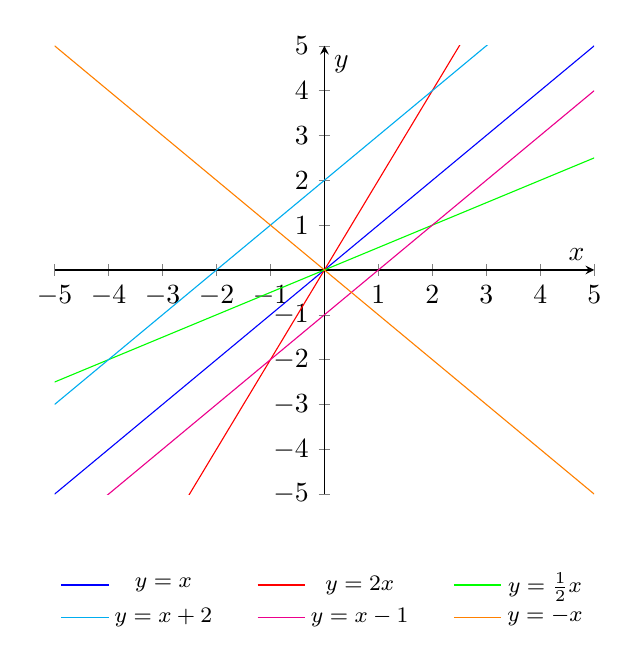
\begin{tikzpicture}
        \begin{axis}[
            axis lines=middle,
            xlabel=$x$,
            ylabel=$y$,
            xmin=-5,
            xmax=5,
            ymin=-5,
            ymax=5,
            xtick={-5,-4,-3,-2,-1,0,1,2,3,4,5},
            ytick={-5,-4,-3,-2,-1,0,1,2,3,4,5},
            legend pos=outer north east,
            legend style={
                draw=none,
                at={(0.5,-0.15)},
                anchor=north,
                legend columns=3,
                font=\footnotesize,
                /tikz/every even column/.append style={column sep=0.5cm},
            },
        ]
        
        % Linear Function: y = x
        \addplot[blue, domain=-5:5, samples=100] {x};
        \addlegendentry{$y = x$}
        
        % Transformed Functions
        \addplot[red, domain=-5:5, samples=100] {2*x};
        \addlegendentry{$y = 2x$}
        
        \addplot[green, domain=-5:5, samples=100] {0.5*x};
        \addlegendentry{$y = \frac{1}{2}x$}
        
        \addplot[cyan, domain=-5:5, samples=100] {x + 2};
        \addlegendentry{$y = x + 2$}
        
        \addplot[magenta, domain=-5:5, samples=100] {x - 1};
        \addlegendentry{$y = x - 1$}

        \addplot[orange, domain=-5:5, samples=100] {-x};
        \addlegendentry{$y = -x$}
        
        \end{axis}
        \end{tikzpicture}
    \end{center}
    \textbf{Definitonsmenge}: $\mathbb{D} = \mathbb{R}$\\
    \textbf{Wertemenge}: $\mathbb{W} = \mathbb{R}$\\
    \textbf{Nullstelle berechnen}\\
    Funktion gleich Null setzen und nach X auflösen.\\
    \textbf{Achsenabschnitt}:\\
    Bei linearen Funktionen lässt sich der y-Achsenabschnitt aus der Funktionsgleichung ablesen: Der y-Achsenabschnitt $y = {\color{red}mx + b}$ von ist $y = {\color{red}b}$\\
    \textbf{Schnittpunkt berechnen}\\
    Beide Funktionen gleichsetzen, nach X auflösen und in eine der beiden Funktionen einsetzen um Y zu berechnen.\\
    \textbf{Umkehrfunktion bilden}\\
    Funktion nach x auflösen, x und y vertauschen.\\
   
% Quadratic Function: y = x^2
\subsection*{Quadratische Funktion}
\begin{center}
    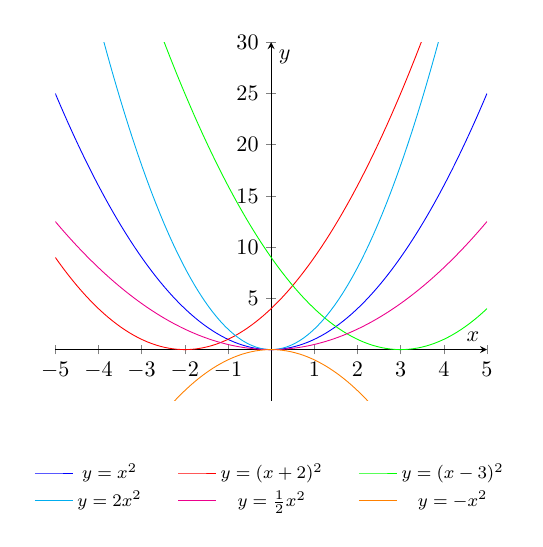
\begin{tikzpicture}[scale=0.8]
    \begin{axis}[
        axis lines=middle,
        xlabel=$x$,
        ylabel=$y$,
        xmin=-5,
        xmax=5,
        ymin=-5,
        ymax=30,
        xtick={-5,-4,-3,-2,-1,0,1,2,3,4,5},
        ytick={0,5,10,15,20,25,30},
        legend pos=outer north east,
            legend style={
                draw=none,
                at={(0.5,-0.15)},
                anchor=north,
                legend columns=3,
                font=\footnotesize,
                /tikz/every even column/.append style={column sep=0.5cm},
            },
    ]
    \addplot[blue, domain=-5:5, samples=100] {x^2};
    \addlegendentry{$y = x^2$}
    
    % Transformed Functions
    \addplot[red, domain=-5:5, samples=100] {(x+2)^2};
    \addlegendentry{$y = (x + 2)^2$}
    
    \addplot[green, domain=-5:5, samples=100] {(x-3)^2};
    \addlegendentry{$y = (x - 3)^2$}
    
    \addplot[cyan, domain=-5:5, samples=100] {2*x^2};
    \addlegendentry{$y = 2x^2$}
    
    \addplot[magenta, domain=-5:5, samples=100] {0.5*x^2};
    \addlegendentry{$y = \frac{1}{2}x^2$}

    \addplot[orange, domain=-5:5, samples=100] {-x^2};
    \addlegendentry{$y = -x^2$}
    
    \end{axis}
    \end{tikzpicture}
    \end{center}
    \textbf{Definitonsmenge}: $\mathbb{D} = \mathbb{R}$\\
    \textbf{Wertemenge}: $\mathbb{W} = \{y \in \mathbb{R} | y \geq 0\}$\\
    Der Graph einer quadratischen Funktion ist eine Parabel.
    Der tiefste oder höchste Punkt einer Parabel heisst Scheitelpunkt.\\
    \textbf{Achsenabschnitt}:\\
    Die x-Koordinate des Schnittpunktes mit der y-Achse ist immer Null.
    Bei quadratischen Funktionen lässt sich der y-Achsenabschnitt aus der Funktionsgleichung ablesen: Der y-Achsenabschnitt $y = ax^2 + bx + {\color{red}c}$ von ist $y = {\color{red}c}$
    \textbf{Nullstellen berechnen}:\\
    Funktionsgleichung gleich Null setzen, Gleichung lösen.
    
    % Exponential Function: y = 2^x
    \subsection*{Exponential Funktion}
    \begin{center}
    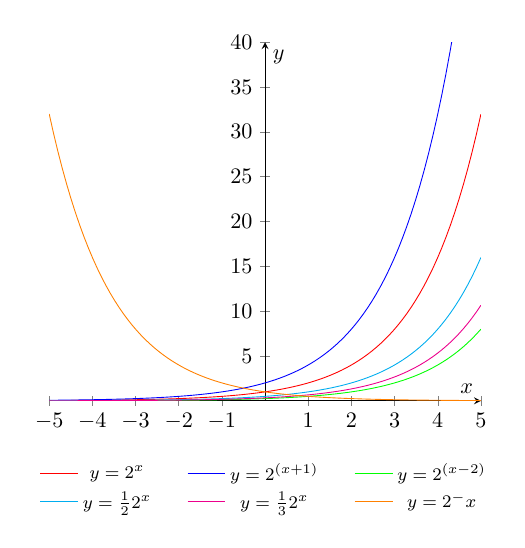
\begin{tikzpicture}[scale=0.8]
    \begin{axis}[
        axis lines=middle,
        xlabel=$x$,
        ylabel=$y$,
        xmin=-5,
        xmax=5,
        ymin=0,
        ymax=40,
        xtick={-5,-4,-3,-2,-1,0,1,2,3,4,5},
        ytick={0,5,10,15,20,25,30,35,40},
        legend pos=outer north east,
            legend style={
                draw=none,
                at={(0.5,-0.15)},
                anchor=north,
                legend columns=3,
                font=\footnotesize,
                /tikz/every even column/.append style={column sep=0.5cm},
            },
    ]
    \addplot[red, domain=-5:5, samples=100] {2^x};
    \addlegendentry{$y = 2^x$}
    
    % Transformed Functions
    \addplot[blue, domain=-5:5, samples=100] {2^(x+1)};
    \addlegendentry{$y = 2^{(x + 1)}$}
    
    \addplot[green, domain=-5:5, samples=100] {2^(x-2)};
    \addlegendentry{$y = 2^{(x - 2)}$}
    
    \addplot[cyan, domain=-5:5, samples=100] {0.5*2^x};
    \addlegendentry{$y = \frac{1}{2}2^x$}
    
    \addplot[magenta, domain=-5:5, samples=100] {2^x / 3};
    \addlegendentry{$y = \frac{1}{3}2^x$}

    \addplot[orange, domain=-5:5, samples=100] {2^-x};
    \addlegendentry{$y = 2^-x$}
    
    \end{axis}
    \end{tikzpicture}
    \end{center}
    \textbf{Definitonsmenge}: $\mathbb{D} = \mathbb{R}$\\
    \textbf{Wertemenge}: $\mathbb{W} = \mathbb{R^+}$\\
    \textbf{Basis a zwisschen 0 und 1}\\
    Gilt $0 < a < 1$, so ist die Exponentialfunktion streng monoton fallend. Exponentialler Abnahme.\\
    \textbf{Basis a grösser 1}\\
    Gilt $a > 1$, so ist die Exponentialfunktion streng monoton wachsend. Exponentielles Wachstum.\\
    \textbf{Eigenschaften}\\
    Der Graph einer Exponentialfunktion verläuft durch den Punkt $(0;1)$.\\
    Die Exponentialfunktion hat keine Nullstelle.\\
    Die x-Achse ist eine waagrechte Asymptote die beliebig nah an den Nullpunkt kommt.\\
    \textbf{Umkehrfunktion}\\
    Die Umkehrfunktion der Exponentialfunktion heisst Logarithmusfunktion. $f(x) = \log_{a}x$\\ 
        
    \subsection*{Logarithmische Funktion}
    % Logarithmic Function: y = ln(x)
    \begin{center}
    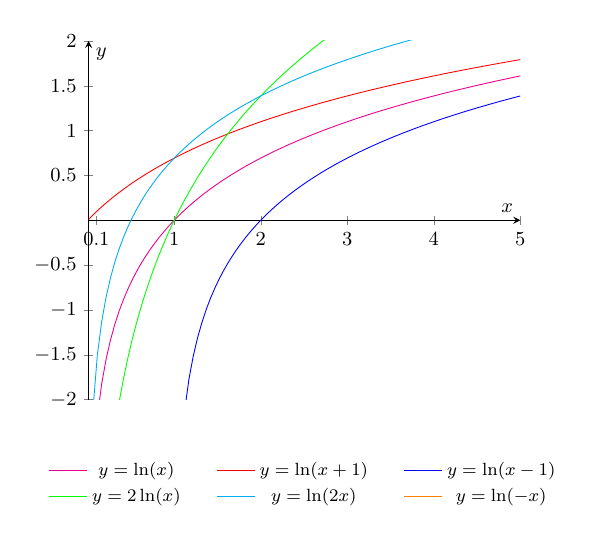
\begin{tikzpicture}[scale=0.8]
    \begin{axis}[
        axis lines=middle,
        xlabel=$x$,
        ylabel=$y$,
        xmin=0.01,
        xmax=5,
        ymin=-2,
        ymax=2,
        xtick={0.01,0.1,1,2,3,4,5},
        ytick={-2,-1.5,-1,-0.5,0,0.5,1,1.5,2},
        legend pos=outer north east,
            legend style={
                draw=none,
                at={(0.5,-0.15)},
                anchor=north,
                legend columns=3,
                font=\footnotesize,
                /tikz/every even column/.append style={column sep=0.5cm},
            },
    ]
    \addplot[magenta, domain=0.01:5, samples=100] {ln(x)};
    \addlegendentry{$y = \ln(x)$}
    
    % Transformed Functions
    \addplot[red, domain=0.01:5, samples=100] {ln(x+1)};
    \addlegendentry{$y = \ln(x + 1)$}
    
    \addplot[blue, domain=0.01:5, samples=100] {ln(x-1)};
    \addlegendentry{$y = \ln(x - 1)$}
    
    \addplot[green, domain=0.01:5, samples=100] {2*ln(x)};
    \addlegendentry{$y = 2\ln(x)$}
    
    \addplot[cyan, domain=0.01:5, samples=100] {ln(2*x)};
    \addlegendentry{$y = \ln(2x)$}

    \addplot[orange, samples=100] {ln(-x)};
    \addlegendentry{$y = \ln(-x)$}
    \small
    \end{axis}
    \end{tikzpicture}
    \end{center}
    \textbf{Definitonsmenge}: $\mathbb{D} = \mathbb{R^+}$\\
    \textbf{Wertemenge}: $\mathbb{W} = \mathbb{R}$\\
    \textbf{Basis a zwisschen 0 und 1}\\
    Gilt $0 < a < 1$, so ist die Exponentialfunktion streng monoton fallend.\\
    \textbf{Basis a grösser 1}\\
    Gilt $a > 1$, so ist die Exponentialfunktion streng monoton wachsend. Exponentielles Wachstum.\\
    \textbf{Eigenschaften}\\
    Logarithmuskurven verlaufen durch den Punkt $(1;0)$.    Die Nullstellen der Logarithmusfunktionen ist x=1.\\
    Logarithmuskurven verlaufen rechts der y-Achse.\\
    Logarithmusfunktionen haben keinen y-Achsenabschnitt.\\
    Die y-Achse ist eine senkrechte Asymptote die beliebig nah an den Nullpunkt kommt.\\
    \subsection*{Potenz Funktion}
    \subsubsection*{Potenzfunktionen mit Positiven Exponenten}
    \subsubsection*{Definition}
    Eine Funktion $f$ mit der Funktionsgleichung $f(x) = x^n \quad \text{ mit } n \in \mathbb{Z}\setminus\{0\}$ heisst Potenzfunktion. \\~\\
    \subsubsection*{Gerade Exponenten}
    Als Beispiele dienen die Funktionen $f(x) = x^2$ und $f(x) = x^4$. \\
    Um die Graphen besser zu zeichnen, berechnen wir zunächst einige Funktionswerte:
    \[\begin{array}{r|c|c|c|c|c|c|c} x & -1{,}5 & {\color{blue}-1} & -0{,}5 & {\color{blue}0} & 0{,}5 & {\color{blue}1} & 1{,}5 \\ \hline x^2 & 2{,}25 & {\color{blue}1} & 0{,}25 & {\color{blue}0} & 0{,}25 & {\color{blue}1} & 2{,}25 \\ \hline x^4 & 5{,}0625 & {\color{blue}1} & 0{,}0625 & {\color{blue}0} & 0{,}0625 & {\color{blue}1} & 5{,}0625 \end{array}\]
    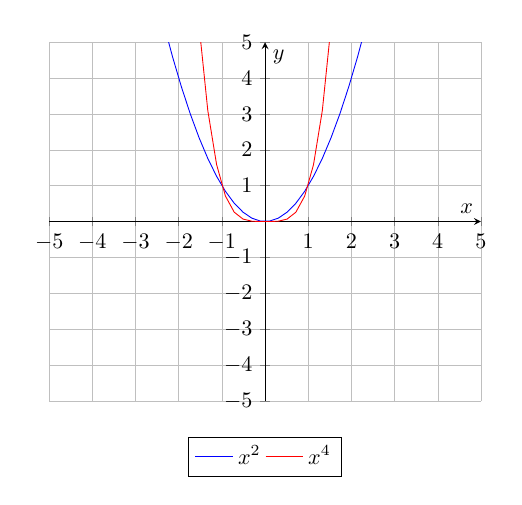
\begin{tikzpicture}[scale=0.8]
        \begin{axis}[
                xlabel=$x$,
                ylabel=$y$,
                xmax=5,
                xmin=-5,
                ymax=5,
                ymin=-5,
                axis x line=middle,
                axis y line=middle,
                legend style={at={(0.5,-0.1)},
                        anchor=north,legend columns=-1},
                grid=major,
                grid style={line width=.1pt, draw=gray!10},
                major grid style={line width=.2pt,draw=gray!50},
                xtick={-5,-4,-3,-2,-1,0,1,2,3,4,5},
                ytick={-5,-4,-3,-2,-1,0,1,2,3,4,5},
                samples=50
            ]
            \addplot [blue] {x^2};
            \addlegendentry {$x^2$};
            \addplot [red] {x^4};
            \addlegendentry {$x^4$};


        \end{axis}
    \end{tikzpicture}
    \subsubsection*{Ungerade Exponenten}
    Als Beispiele dienen die Funktionen $f(x) = x^3$ und $f(x) = x^5$. \\
    Um die Graphen besser zu zeichnen, berechnen wir zunächst einige Funktionswerte:  \\
    \footnotesize
    \[\begin{array}{r|c|c|c|c|c|c|c} x & -1{,}5 & {\color{blue}-1} & -0{,}5 & {\color{blue}0} & 0{,}5 & {\color{blue}1} & 1{,}5 \\ \hline x^3 & -3{,}375 & {\color{blue}-1} & -0{,}125 & {\color{blue}0} & 0{,}125 & {\color{blue}1} & 3{,}375 \\ \hline x^5 & -7{,}59375 & {\color{blue}-1} & 0{,}03125 & {\color{blue}0} & 0{,}03125 & {\color{blue}1} & 7{,}59375 \end{array}\]
    \normalsize
    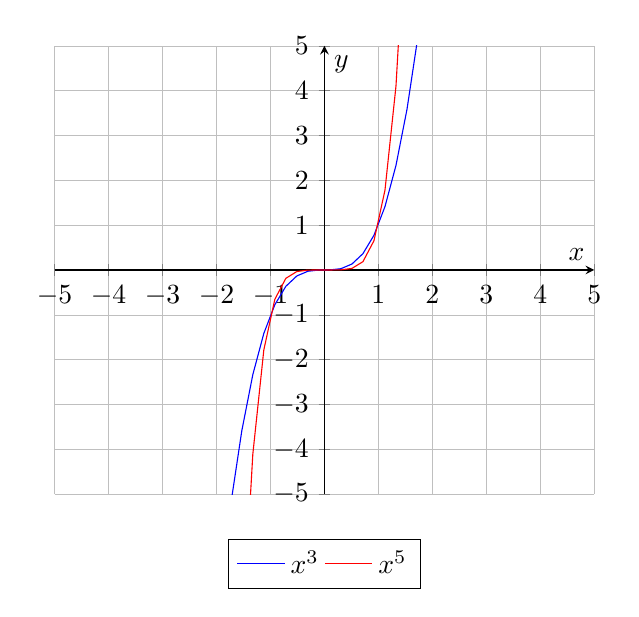
\begin{tikzpicture}%[scale=1.5]
        \begin{axis}[
                xlabel=$x$,
                ylabel=$y$,
                xmax=5,
                xmin=-5,
                ymax=5,
                ymin=-5,
                restrict y to domain=-10:10,
                axis x line=middle,
                axis y line=middle,
                legend style={at={(0.5,-0.1)},
                        anchor=north,legend columns=-1},
                grid=major,
                grid style={line width=.1pt, draw=gray!10},
                major grid style={line width=.2pt,draw=gray!50},
                xtick={-5,-4,-3,-2,-1,0,1,2,3,4,5},
                ytick={-5,-4,-3,-2,-1,0,1,2,3,4,5},
                samples=50
            ]
            \addplot [blue] {x^3};
            \addlegendentry {$x^3$};
            \addplot [red] {x^5};
            \addlegendentry {$x^5$};
        \end{axis}
    \end{tikzpicture}

    \subsubsection*{Zusammenfassung der wichtigsten Eigenschaften}
    Potenzfunktionen mit positiven ganzzahligen Exponenten $\boldsymbol{f(x) = x^n}$ haben folgende Eigenschaften: \\
    \begin{tabularx}{\columnwidth} {
            | >{\raggedright\arraybackslash}X
            | >{\raggedright\arraybackslash}X
            | >{\raggedright\arraybackslash}X |}
        \hline
                          & \textbf{n gerade}                 & \textbf{n ungerade}       \\ \hline
        D-Menge  & $\mathbb{D} = \mathbb{R}$         & $\mathbb{D} = \mathbb{R}$ \\ \hline
        Wertemenge        & $\mathbb{W} = \mathbb{R}^{+}_{0}$ & $\mathbb{W} = \mathbb{R}$ \\ \hline
        Symmetrie         & achsen                 & punkt           \\
                          & zur y-ache                        & zum K-Ursprung            \\ \hline
        Gemeinsame  & $(-1,1)$,$(0|0)$,      & $(-1,-1)$,$(0|0)$, \\ 
        Punkte& $(1|1)$          & $(1|1)$ \\ \hline
    \end{tabularx}
    \subsection*{Potenzfunktionen mit negativen Exponenten}
    Die Graphen von Potenzfunktionen heissen Hyperbeln n-ter Ordnung, wenn der Exponent negativ ist.
    \subsubsection*{Gerade Exponenten}
     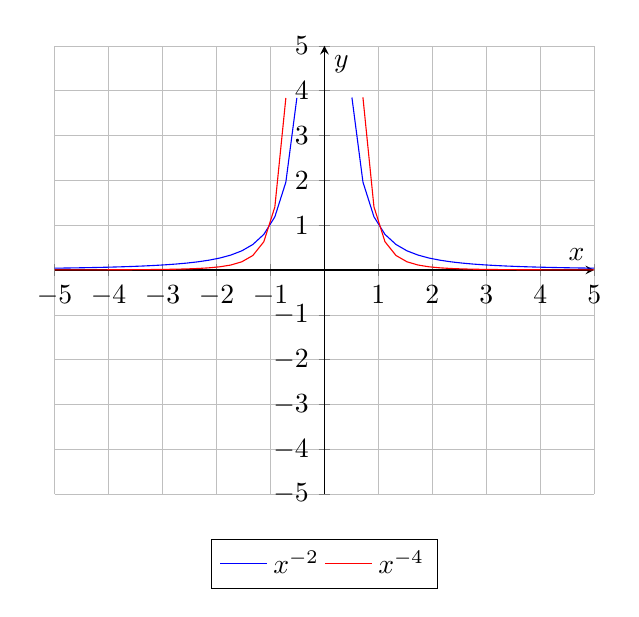
\begin{tikzpicture}[scale=1]
        \begin{axis}[
                xlabel=$x$,
                ylabel=$y$,
                xmax=5,
                xmin=-5,
                ymax=5,
                ymin=-5,
                restrict y to domain=-10:10,
                axis x line=middle,
                axis y line=middle,
                legend style={at={(0.5,-0.1)},
                        anchor=north,legend columns=-1},
                grid=major,
                grid style={line width=.1pt, draw=gray!10},
                major grid style={line width=.2pt,draw=gray!50},
                xtick={-5,-4,-3,-2,-1,0,1,2,3,4,5},
                ytick={-5,-4,-3,-2,-1,0,1,2,3,4,5},
                samples=50
            ]
            \addplot [blue] {x^-2};
            \addlegendentry {$x^{-2}$};
            \addplot [red] {x^-4};
            \addlegendentry {$x^{-4}$};
        \end{axis}
    \end{tikzpicture}\\
    Als Beispiele dienen die Funktionen $f(x) = x^{-2}$ und $f(x) = x^{-4}$. \\
    Um die Graphen besser zu zeichnen, berechnen wir zunächst einige Funktionswerte: \\~\\
    $\begin{array}{r|c|c|c|c|c|c} x & -1{,}5 & {\color{blue}-1} & -0{,}5 & 0{,}5 & {\color{blue}1} & 1{,}5 \\ \hline x^{-2} & 0{,}\bar{4} & {\color{blue}1} & 4 & 4 & {\color{blue}1} & 0{,}\bar{4} \\ \hline x^{-4} & \approx 0{,}1975 & {\color{blue}1} & 16 & 16 & {\color{blue}1} & \approx 0{,}1975 \end{array}$ \\~\\
    \small
    \subsubsection*{Gerade Exponenten}
    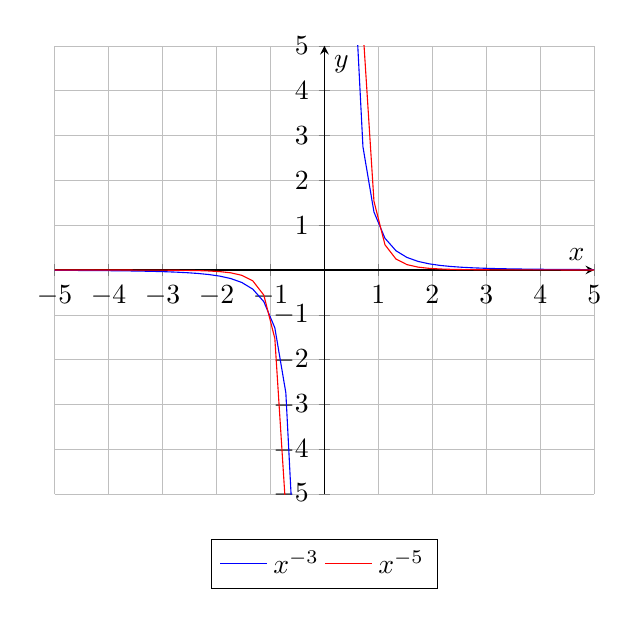
\begin{tikzpicture}[scale=1]
        \begin{axis}[
                xlabel=$x$,
                ylabel=$y$,
                xmax=5,
                xmin=-5,
                ymax=5,
                ymin=-5,
                restrict y to domain=-10:10,
                axis x line=middle,
                axis y line=middle,
                legend style={at={(0.5,-0.1)},
                        anchor=north,legend columns=-1},
                grid=major,
                grid style={line width=.1pt, draw=gray!10},
                major grid style={line width=.2pt,draw=gray!50},
                xtick={-5,-4,-3,-2,-1,0,1,2,3,4,5},
                ytick={-5,-4,-3,-2,-1,0,1,2,3,4,5},
                samples=50
            ]
            \addplot [blue] {x^-3};
            \addlegendentry {$x^{-3}$};
            \addplot [red] {x^-5};
            \addlegendentry {$x^{-5}$};
        \end{axis}
    \end{tikzpicture}\\
    Als Beispiele dienen die Funktionen $f(x) = x^{-3}$ und $f(x) = x^{-5}$. \\
    Um die Graphen besser zu zeichnen, berechnen wir zunächst einige Funktionswerte: \\~\\
    $\begin{array}{r|c|c|c|c|c|c} x & -1{,}5 & {\color{blue}-1} & -0{,}5 & 0{,}5 & {\color{blue}1} & 1{,}5 \\ \hline x^{-3} & \approx -0{,}2963 & {\color{blue}-1} & -8 & 8 & {\color{blue}1} & \approx 0{,}2963 \\ \hline x^{-5} & \approx -0{,}1317 & {\color{blue}-1} & -32 & 32 & {\color{blue}1} & \approx 0{,}1317 \end{array}$ \\~\\
 

    \subsubsection*{Zusammenfassung der wichtigsten Eigenschaften}
    Potenzfunktionen mit negativen ganzzahligen Exponenten $\boldsymbol{f(x) = x^{-n}}$ haben folgende Eigenschaften: \\\\
    \begin{tabularx}{\columnwidth} {
            | >{\raggedright\arraybackslash}X
            | >{\raggedright\arraybackslash}X
            | >{\raggedright\arraybackslash}X |}
        \hline
                          & \textbf{n gerade}                       & \textbf{n ungerade}                     \\ \hline
        D-Menge  & $\mathbb{D} = \mathbb{R}\setminus\{0\}$ & $\mathbb{D} = \mathbb{R}\setminus\{0\}$ \\ \hline
        Wertemenge        & $\mathbb{W} = \mathbb{R}^{+}$           & $\mathbb{W} = \mathbb{R}\setminus\{0\}$ \\ \hline
        Symmetrie         & achsen                       & punkt                         \\
                          & zur y-ache                              & zum K-Ursprung                          \\ \hline
        Gemeinsame Punkte & $(-1,1)$,$(1|1)$                        & $(-1,-1)$,$(1|1)$                       \\ \hline
        Asymptoten        & x-Achse, y-Achse                        & x-Achse, y-Achse                        \\ \hline
    \end{tabularx}


    
    \subsection*{Wurzel Funktion}
    % Square Root Function: y = sqrt(x)
    \begin{center}
    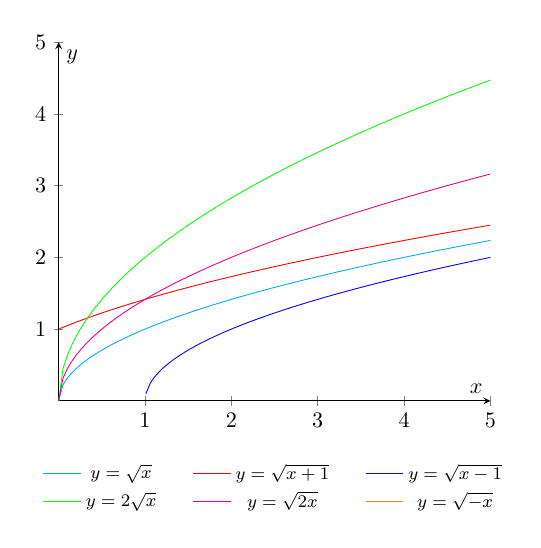
\begin{tikzpicture}[scale=0.8]
    \begin{axis}[
        axis lines=middle,
        xlabel=$x$,
        ylabel=$y$,
        xmin=0,
        xmax=5,
        ymin=0,
        ymax=5,
        xtick={0,1,2,3,4,5},
        ytick={0,1,2,3,4,5},
        legend pos=outer north east,
            legend style={
                draw=none,
                at={(0.5,-0.15)},
                anchor=north,
                legend columns=3,
                font=\footnotesize,
                /tikz/every even column/.append style={column sep=0.5cm},
            },
    ]
    \addplot[cyan, domain=0:5, samples=100] {sqrt(x)};
    \addlegendentry{$y = \sqrt{x}$}
    
    % Transformed Functions
    \addplot[red, domain=0:5, samples=100] {sqrt(x+1)};
    \addlegendentry{$y = \sqrt{x + 1}$}
    
    \addplot[blue, domain=0:5, samples=100] {sqrt(x-1)};
    \addlegendentry{$y = \sqrt{x - 1}$}
    
    \addplot[green, domain=0:5, samples=100] {2*sqrt(x)};
    \addlegendentry{$y = 2\sqrt{x}$}
    
    \addplot[magenta, domain=0:5, samples=100] {sqrt(2*x)};
    \addlegendentry{$y = \sqrt{2x}$}

    \addplot[orange, domain=0:5, samples=100] {sqrt(-x)};
    \addlegendentry{$y = \sqrt{-x}$}
    
    \end{axis}
    \end{tikzpicture}
    \end{center}
    \textbf{Definition ungerader Wurzelexponent}\\
    \textbf{Definitonsmenge}: $\mathbb{D} = \mathbb{R^+}$\\
    \textbf{Wertemenge}: $\mathbb{W} = \mathbb{R^+}$\\
    \textbf{Definition gerader Wurzelexponent}\\
    \textbf{Definitonsmenge}: $\mathbb{D} = \mathbb{R}$\\
    \textbf{Wertemenge}: $\mathbb{W} = \mathbb{R}$\\

    % Absolute Value Function: y = |x|

    \subsection*{Betragsfunktion}
    \begin{center}
    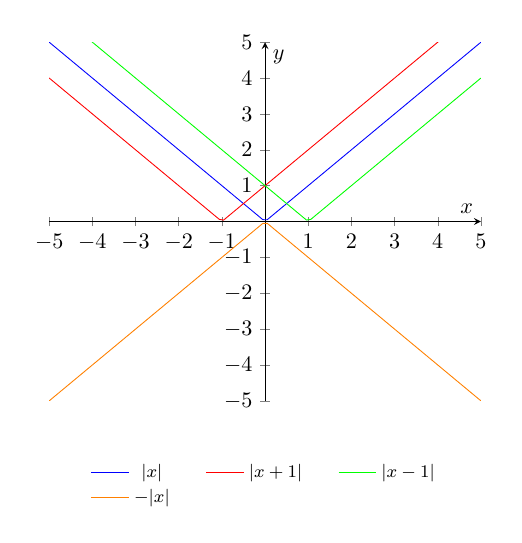
\begin{tikzpicture}[scale=0.8]
    \begin{axis}[
        axis lines=middle,
        xlabel=$x$,
        ylabel=$y$,
        xmin=-5,
        xmax=5,
        ymin=-5,
        ymax=5,
        xtick={-5,-4,-3,-2,-1,0,1,2,3,4,5},
        ytick={-5,-4,-3,-2,-1,0,1,2,3,4,5},
        legend pos=outer north east,
        legend style={
            draw=none,
            at={(0.5,-0.15)},
            anchor=north,
            legend columns=3,
            font=\footnotesize,
            /tikz/every even column/.append style={column sep=0.5cm},
        },
    ]
    
    \addplot[samples=100,blue]{abs(x)};
            \addlegendentry {$|x|$};
            \addplot[samples=100,red]{abs(x+1)};
            \addlegendentry {$|x+1|$};
            \addplot[samples=100,green]{abs(x-1)};
            \addlegendentry {$|x-1|$};
            \addplot[samples=100,orange]{-abs(x)};
            \addlegendentry {$-|x|$};
    
    \end{axis}
    \end{tikzpicture}
    \end{center}
    \begin{center}
        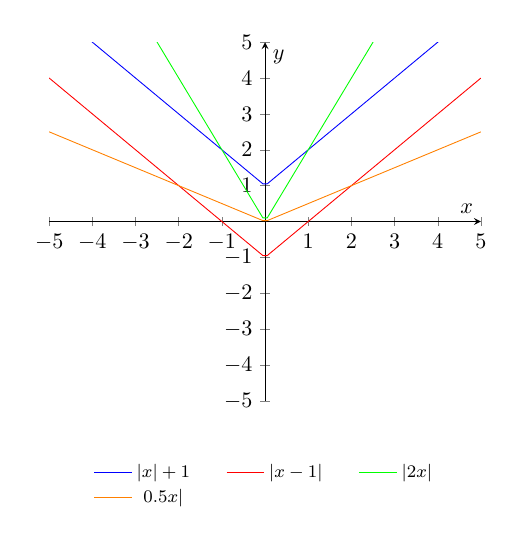
\begin{tikzpicture}[scale=0.8]
        \begin{axis}[
            axis lines=middle,
            xlabel=$x$,
            ylabel=$y$,
            xmin=-5,
            xmax=5,
            ymin=-5,
            ymax=5,
            xtick={-5,-4,-3,-2,-1,0,1,2,3,4,5},
            ytick={-5,-4,-3,-2,-1,0,1,2,3,4,5},
            legend pos=outer north east,
            legend style={
                draw=none,
                at={(0.5,-0.15)},
                anchor=north,
                legend columns=3,
                font=\footnotesize,
                /tikz/every even column/.append style={column sep=0.5cm},
            },
        ]
        
        \addplot[samples=100,blue]{abs(x)+1};
        \addlegendentry {$|x|+1$};
        \addplot[samples=100,red]{abs(x)-1};
        \addlegendentry {$|x-1|$};
        \addplot[samples=100,green]{abs(2*x)};
        \addlegendentry {$|2x|$};
        \addplot[samples=100,orange]{abs(0.5*x)};
        \addlegendentry {$0.5x|$};
        
        \end{axis}
        \end{tikzpicture}
        \end{center}

        \subsection*{Gebrochenrationale Funktionen}
      
        \textbf{Definitionsmenge}\\
         $\mathbb{D}_f = \mathbb{R}\setminus\{\text{Nullstellen der Nennerfunktion}\}$
        \subsubsection*{Senkrechte Asymptote}
        Eine senkrechte Gerade, der sich eine Kurve bei deren immer grösser werdender Entfernung vom Koordinatenursprung unbegrenzt nähert, heisst senkrechte Asymptote.\\
        \textbf{Bedingung}\\
        Bedingung für die Existenz einer senkrechten Asymptote ist, dass die Nennerfunktion (mindestens) eine Nullstelle hat:
        \textbf{Anleitung}
        Funktionsgleichung der Nennerfunktion gleich Null setzen: \\
        $f(x) = \frac{1}{x-1} \Longrightarrow x - 1 = 0$  \\
        Gleichung lösen: $x = 1$ \\
        Die senkrechte Asymptote verlauft durch x = 1.
         
        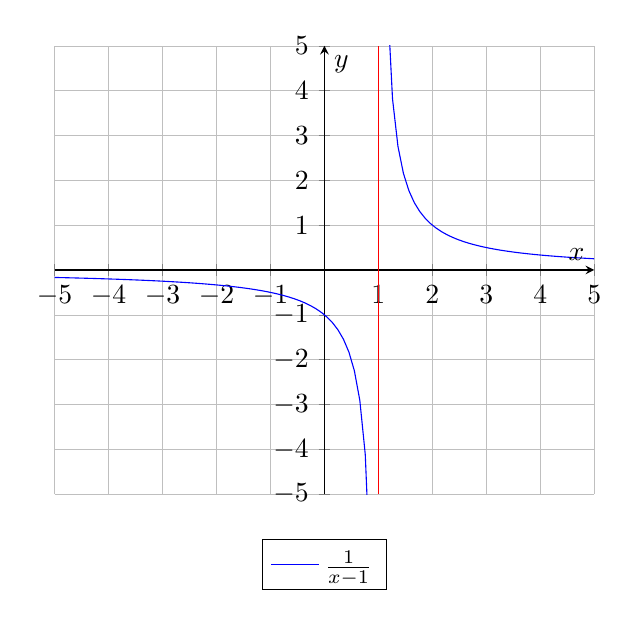
\begin{tikzpicture}%[scale=1.0]
            \begin{axis}[
                    xlabel=$x$,
                    ylabel=$y$,
                    xmax=5,
                    xmin=-5,
                    ymax=5,
                    ymin=-5,
                    axis x line=middle,
                    axis y line=middle,
                    legend style={at={(0.5,-0.1)},
                            anchor=north,legend columns=-1},
                    grid=major,
                    grid style={line width=.1pt, draw=gray!10},
                    major grid style={line width=.2pt,draw=gray!50},
                    xtick={-5,-4,-3,-2,-1,0,1,2,3,4,5},
                    ytick={-5,-4,-3,-2,-1,0,1,2,3,4,5},
                    samples=50
                ]
                \addplot[samples=100,domain=-5:5,blue,restrict y to domain=-15:15]{1/(x-1)};
                \addlegendentry {$\frac{1}{x-1}$};
                \draw[red] ({axis cs:1,0}|-{rel axis cs:0,0}) -- ({axis cs:1,0}|-{rel axis cs:0,1});
                \addlegendentry {$x=1$};
    
            \end{axis}
        \end{tikzpicture}\\
        \subsubsection*{Waagrechte Asymptote}
        Eine waagrechte Gerade, der sich eine Kurve bei deren immer groesser werdender Entfernung vom Koordinatenursprung unbegrenzt nähert, heisst waagrechte Asymptote.
        \textbf{Bedingung}\\
        Eine gebrochenrationale Funktion:
        \[y = \frac{{\color{red}a_n} x^{\fcolorbox{red}{white}{$n$}} + a_{n-1} x^{n-1} + \dots + a_1 x + a_ 0}{{\color{red}b_m} x^{\fcolorbox{red}{white}{$m$}} + b_{m-1} x^{m-1} + \dots + b_1 x + b_ 0}\]
        besitzt eine waagrechte Asymptote, wenn: \\
        Zählergrad < Nennergrad (n < m) dann: Die x-Achse ist die waagrechte Asymptote \\
        Zählergrad = Nennergrad (n = m) dann:  Die zur x-Achse parallele Gerade mit der Gleichung $y = {\color{red}\frac{a_n}{b_m}}$ ist die waagrechte Asymptote.
        \textbf{Anleitung}\\
        Zählergrad und Nennergrad bestimmen: \\
        Da der Zählergrad (0) kleiner ist als der Nennergrad (1), besitzt die gebrochenrationale Funktion eine waagrechte Asymptote.
        Waagrechte Asymptote berechnen: \\
        Wegen Zählergrad < Nennergrad ist die x-Achse die waagrechte Asymptote.
        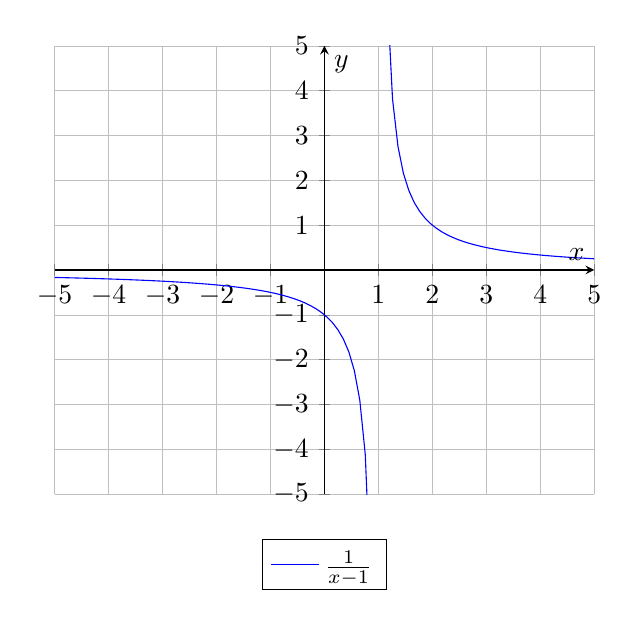
\begin{tikzpicture}%[scale=1.0]
            \begin{axis}[
                    xlabel=$x$,
                    ylabel=$y$,
                    xmax=5,
                    xmin=-5,
                    ymax=5,
                    ymin=-5,
                    axis x line=middle,
                    axis y line=middle,
                    legend style={at={(0.5,-0.1)},
                            anchor=north,legend columns=-1},
                    grid=major,
                    grid style={line width=.1pt, draw=gray!10},
                    major grid style={line width=.2pt,draw=gray!50},
                    xtick={-5,-4,-3,-2,-1,0,1,2,3,4,5},
                    ytick={-5,-4,-3,-2,-1,0,1,2,3,4,5},
                    samples=50
                ]
                \addplot[samples=100,domain=-5:5,blue,restrict y to domain=-15:15]{1/(x-1)};
                \addlegendentry {$\frac{1}{x-1}$};
            \end{axis}
        \end{tikzpicture}\\
    \normalsize
    

    \newpage
\end{multicols}